\documentclass[manuscript,screen,review]{acmart}

\newcommand{\HRule}{\rule{\linewidth}{0.5mm}} 							% horizontal line and its thickness

\newcommand{\rev}[1]{\color{red}[#1]\color{black}\xspace}

\newcommand{\method}[1]{\textbf{#1}.}

%%%%%%%%%%%%%% math defs %%%%%%%%%%%%%%%%%%%%%
% trajectory
\newcommand{\traj}{\tau}
\newcommand{\point}{x}
\newcommand{\ts}{t}
\newcommand{\timePeriod}{t_{max}}
\newcommand{\nDims}{n}
\newcommand{\nPoints}{m}
\newcommand{\trajSet}{T}
\newcommand{\distTrajTraj}[2]{d_{\trajSet}(#1, #2)}

% embedding/encoding
\newcommand{\emb}{\epsilon}
\newcommand{\embDims}{p}
\newcommand{\embSet}{E}
\newcommand{\embFunc}{\Phi}
\newcommand{\distEmbEmb}[2]{d_{\embSet}(#1, #2)}


\newcommand{\realSet}[1]{\mathbb{R}^{#1}}
%%%%%%%% CREATE DOCUMENT STRUCTURE %%%%%%%%
%% Language and font encodings
\usepackage[english]{babel}
\usepackage[utf8x]{inputenc}
\usepackage[T1]{fontenc}
%\usepackage{subfig}

%% Sets page size and margins
%\usepackage[a4paper,top=3cm,bottom=2cm,left=2cm,right=2cm,marginparwidth=1.75cm]{geometry}

%% Useful packages
\usepackage{amsmath}
\usepackage{bm}
%\usepackage{amssymb} % Fancy math letters for sets
\usepackage{graphicx}
%\usepackage[colorlinks=true, allcolors=blue]{hyperref}

\usepackage{blindtext}
\usepackage{natbib}
\usepackage{xcolor} % I like colours

\usepackage{glossaries} % Acronyms

\usepackage{tabulary}
\usepackage{booktabs} % fancy table rules
%%%%%%%%% general acronyms
\newacronym[longplural={Degrees of Freedom}]{dof}{DoF}{Degree of Freedom}

%%%%%%%%% general ML acronyms

\newacronym{a3c}{A3C}{Asynchronous Advantage Actor-Critic}

\newacronym{bc}{BC}{Behaviooural Cloning}

\newacronym{cnn}{CNN}{Convolutional Neural Network}
\newacronym{cvae}{cVAE}{conditional Variational Auto-Encoder}

\newacronym{dl}{DL}{Deep Learning}
\newacronym{drl}{DRL}{Deep reinforcement Learning}

\newacronym{kge}{KGE}{Knowledge Graph Embedding}
\newacronym{kde}{KDE}{Kernel Density Estimate}

\newacronym{gan}{GAN}{Generative Adversarial Network}
\newacronym{gnn}{GNN}{Graph Neural Network}
\newacronym{gru}{GRU}{Gated Recurrent Unit}
\newacronym{gmm}{GMM}{Gaussian Mixture Model}
\newacronym{lstm}{LSTM}{Long Short-Term Memory}

\newacronym{nn}{NN}{Neural Network}

\newacronym[longplural=Points of Interest]{poi}{PoI}{Point of Interest}

\newacronym{rnn}{RNN}{Recurrent Neural Network}
\newacronym{rl}{RL}{Reinforcement Learning}

\newacronym{tsne}{t-SNE}{t-Distributed Stochastic Neighbor Embedding}

\newacronym{mlp}{MLP}{Multi-Layer Perceptron}

\newacronym{vae}{VAE}{Variational Auto-Encoder}

%%%%%%%%% numerical methods acronyms

\newacronym{dtw}{DTW}{Dynamic Time Warp}

\newacronym{edr}{EDR}{Edit Distance on Real Sequence}
\newacronym{edwp}{EDwP}{Edit Distance with Projections}
\newacronym{erp}{ERP}{Edit distance with Real Penalty}

\newacronym{fd}{FD}{Fréchet Distance}

\newacronym{hd}{HD}{Hausdorff Distance}

\newacronym{lcss}{LCSS}{Longest Common Subsequence}
\newacronym{lip}{LIP}{Locality In-between Polylines}

\newacronym{owd}{OWD}{One-Way Distance}

%%%%%%%%% social navigation and robots methods acronyms

\newacronym{cs-lstm}{CS-LSTM}{Convolution Social LSTM}

\newacronym{sf}{SF}{Social Force}

\newacronym{lrp}{LRP}{Layer-wise Relevance Propagation}
%%
%% \BibTeX command to typeset BibTeX logo in the docs
\AtBeginDocument{%
	\providecommand\BibTeX{{%
			Bib\TeX}}}

%% Rights management information.  This information is sent to you
%% when you complete the rights form.  These commands have SAMPLE
%% values in them; it is your responsibility as an author to replace
%% the commands and values with those provided to you when you
%% complete the rights form.
\setcopyright{acmlicensed}
\copyrightyear{2018}
\acmYear{2018}
\acmDOI{XXXXXXX.XXXXXXX}

%% These commands are for a PROCEEDINGS abstract or paper.
\acmConference[Conference acronym 'XX]{Make sure to enter the correct
	conference title from your rights confirmation emai}{June 03--05,
	2018}{Woodstock, NY}
%%
%%  Uncomment \acmBooktitle if the title of the proceedings is different
%%  from ``Proceedings of ...''!
%%
%%\acmBooktitle{Woodstock '18: ACM Symposium on Neural Gaze Detection,
	%%  June 03--05, 2018, Woodstock, NY}
\acmISBN{978-1-4503-XXXX-X/18/06}


%%
%% Submission ID.
%% Use this when submitting an article to a sponsored event. You'll
%% receive a unique submission ID from the organizers
%% of the event, and this ID should be used as the parameter to this command.
%%\acmSubmissionID{123-A56-BU3}

%%
%% For managing citations, it is recommended to use bibliography
%% files in BibTeX format.
%%
%% You can then either use BibTeX with the ACM-Reference-Format style,
%% or BibLaTeX with the acmnumeric or acmauthoryear sytles, that include
%% support for advanced citation of software artefact from the
%% biblatex-software package, also separately available on CTAN.
%%
%% Look at the sample-*-biblatex.tex files for templates showcasing
%% the biblatex styles.
%%

%%
%% The majority of ACM publications use numbered citations and
%% references.  The command \citestyle{authoryear} switches to the
%% "author year" style.
%%
%% If you are preparing content for an event
%% sponsored by ACM SIGGRAPH, you must use the "author year" style of
%% citations and references.
%% Uncommenting
%% the next command will enable that style.
%%\citestyle{acmauthoryear}


%%
%% end of the preamble, start of the body of the document source.

\begin{document}


\title{A Survey on Trajectory Encoding Methods for Social Robots}

%%
%% The "author" command and its associated commands are used to define
%% the authors and their affiliations.
%% Of note is the shared affiliation of the first two authors, and the
%% "authornote" and "authornotemark" commands
%% used to denote shared contribution to the research.
\author{Leandro de Souza Rosa}
%\authornote{Both authors contributed equally to this research.}
\email{desouzarosa@diag.uniroma1.it}
\orcid{0000-0003-3457-9164}
\author{Luca Iocchi}
\authornotemark[1]
\email{iocchi@diag.uniroma1.it}
\affiliation{%
  \institution{La Sapienza University of Roma}
  \city{Rome}
  \country{Italy}
}
\author{Julian F. Schumann}
\orcid{0000-0002-4482-5122}
\email{j.f.schumann@tudelft.nl}
\affiliation{%
  \institution{Delft University of Technology}
  \city{Delft}
  \country{Netherlands}
}
\author{Anna Mészáros}
\orcid{0000-0002-8580-9612}
\email{A.Meszaros@tudelft.nl}
\affiliation{%
	\institution{Delft University of Technology}
	\city{Delft}
	\country{Netherlands}
}


\renewcommand{\shortauthors}{de Souza Rosa et al.}


%\section{Abstract}\label{sec: abstract}

\received{20 February 2007}
\received[revised]{12 March 2009}
\received[accepted]{5 June 2009}

%%
%% This command processes the author and affiliation and title
%% information and builds the first part of the formatted document.
\maketitle

\rev{Change table for 1st-encoder, 2nd-encoder ... 4th-encoder + multi-agent encoder, instead of having encoder and assistent}

\rev{copy bib files to single one}

\begin{itemize}
    
    \item Related works
    \begin{itemize}
        \item Other surveys 
    \end{itemize}

    \item Different Encodings
    \begin{itemize}
        \item mlp
        \item rnn
        \begin{itemize}
            \item lstm
            \item gru
        \end{itemize}
        \item self-attention
        \item gnn
        \item cnn
        
        \item misc
        \begin{itemize}
            \item svms
            \item pca
            \item polylines (bezier curves)
            \item rough path signature?
            \item shapelets?
        \end{itemize}
    \end{itemize}

    \item multi-encodings \rev{is this the same as multi-layers?}
	\item Multi-layer
	\begin{itemize}
		\item attention
		\item gmm
		\item cnn
	\end{itemize}

	\item Multi-Agents
	1xn, nxn, 
	\begin{itemize}
		\item max-pooling
		\item gmm
		\item ...
	\end{itemize}

    \item Applications
        \begin{itemize}
            \item Human trajectory prediction
            \item Anomaly detection
            \item Path planning
            \item 
        \end{itemize}

    \item Human side
    \begin{itemize}
        \item Comfort
        \item safety
        \item ...
    \end{itemize}

    \item ?databases, benchmarks, simulators?
\end{itemize}
\section{Abstract}\label{sec: abstract}
\section{Introduction}\label{sec: introduction}

\begin{figure}[h]
	\centering
	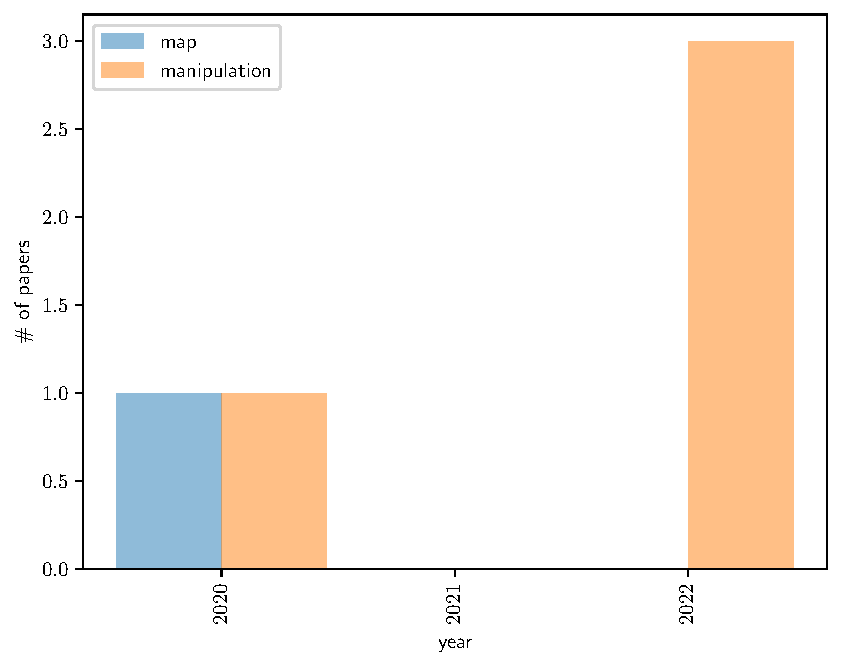
\includegraphics[width=0.7\linewidth]{images/Scope}
	\caption{Number of publications according to Scope.}
	\label{fig:human}
\end{figure}

\section{Related Works}\label{sec: related works}

\section{Encodings}\label{sec: encodings}

\subsection{Recurrent Neural Networks}

\rev{just for testing} \cite{xu2022socialvae} The paper uses relatively normal combination of rnn and attention to encode the past, its most important contribution comes in the recursive reasoning of the decoder.

\subsection{Long-Short Term Memory}

\rev{just for testing} \cite{tsai2020generative} focus on learning human-compliant behaviors for robots navigating in human crowded environments, by optimizing trajectories both for comfort (the absence of annoyance and stress for humans) and naturalness (the similarity between robots and humans).

They state ``reinforcement learning approaches tend to optimize on the comfort aspect of the socially compliant navigation, whereas the inverse reinforcement learning approaches are designed to achieve natural behavior.''

A \gls{lstm} encoder-decoder is defined for each of three social-interaction force (intention, social interaction and fluctuation) from \cite{helbing1995social} to improves interpretability, which are used with a adversarial training to reduce the data-bias tendency of \glspl{lstm}.

The trajectories of the robot and other agents (humans) are encoded with \glspl{lstm}, for intention just the robot trajectory is encoded, for social interaction and fluctuation all trajectories are encoded and passed through a \texttt{maxpooling} layer before the \gls{lstm}.
%
Both encoding are passed to an adversarial training using demonstrations.

\subsection{Graph Neural Networks}

\rev{just for testing} \cite{da2022path} In this paper, they suggest PAGA, which is an improvement on LaneCGNB \cite{liang2020learning}. Namely, the update the method for calculating the attention weights in the GNN used to encode the map. Instead of simply using an the four different adjacency matrices, the replaces that with a more complex matrix able to include connection via intermediate steps.

\section{Multi-Layers}\label{sec: multi-layers}
\section{Multi-Agents}\label{sec: multi-agents}
\section{Applications}\label{sec: applications}
\section{Human Aspects}\label{sec: human aspecs}
\section{Datasets, Benchmarks and Simulators}\label{sec: datasets benchmarks and simulators}

\section{Conclusions}\label{sec: conclusions}
%\section{Comparison}\label{sec: comparison}
%\section{Challenges}\label{sec: challenges}


\begin{acks}
This project has been sponsored by ...
\end{acks}

\bibliographystyle{ACM-Reference-Format}
\bibliography{biblio}
%\bibliography{referencePapers/trajectorySimilarity/numericalMethods/biblio,referencePapers/trajectorySimilarity/clustering/biblio,referencePapers/trajectorySimilarity/trajLearning/biblio,referencePapers/trajectorySimilarity/trajLearningRobotics/biblio,referencePapers/trajectorySimilarity/trajPrediction/biblio,referencePapers/socialNavigation/humanModels/biblio,referencePapers/socialNavigation/pedestrianPrediction/biblio,referencePapers/socialNavigation/socialRobots/biblio,referencePapers/surveys/biblio,referencePapers/datasetsAndBenchmarks/biblio}%

%\appendix

\section{Research Methods}

\subsection{Part One}

Lorem ipsum dolor sit amet, consectetur adipiscing elit. Morbi
malesuada, quam in pulvinar varius, metus nunc fermentum urna, id
sollicitudin purus odio sit amet enim. Aliquam ullamcorper eu ipsum
vel mollis. Curabitur quis dictum nisl. Phasellus vel semper risus, et
lacinia dolor. Integer ultricies commodo sem nec semper.

\subsection{Part Two}

Etiam commodo feugiat nisl pulvinar pellentesque. Etiam auctor sodales
ligula, non varius nibh pulvinar semper. Suspendisse nec lectus non
ipsum convallis congue hendrerit vitae sapien. Donec at laoreet
eros. Vivamus non purus placerat, scelerisque diam eu, cursus
ante. Etiam aliquam tortor auctor efficitur mattis.

\section{Online Resources}

Nam id fermentum dui. Suspendisse sagittis tortor a nulla mollis, in
pulvinar ex pretium. Sed interdum orci quis metus euismod, et sagittis
enim maximus. Vestibulum gravida massa ut felis suscipit
congue. Quisque mattis elit a risus ultrices commodo venenatis eget
dui. Etiam sagittis eleifend elementum.

Nam interdum magna at lectus dignissim, ac dignissim lorem
rhoncus. Maecenas eu arcu ac neque placerat aliquam. Nunc pulvinar
massa et mattis lacinia.


\end{document}
\endinput